%!TEX root=../document.tex

\section{Ergebnisse}
\label{sec:Ergebnisse}

\subsection{CORBA Grundlagen}

\subsection{Installation von JacOrb und OmniORB}
Die Durchf\"uhrung der Aufgabe erfolgte in einer virtuellen Maschiene auf Basis von Debian 8.3 Jessie.
F\"ur die Installation von Java 8 muss das \texttt{jessie-backports} Repository zu der Sources von \texttt{apt} hinzugef\"ugt werden.
Die erfolgt durch Anh\"angen folgender Zeilen an die Datei \texttt{/etc/apt/sources.list}:

\texttt{deb http://httpredir.debian.org/debian jessie-backports main\\
deb-src http://httpredir.debian.org/debian jessie-backports main}

Danach werden die Packetlisten mit \texttt{apt update} aktualisiert.

Vor der eigentlichen Installation der beiden Programme werden nun folgende Packets installiert:
\begin{itemize}
    \item build-essentials
    \item gcc
    \item g++
    \item openjdk-8-jdk
    \item ant
    \item make
\end{itemize}

Um tats\"achlich Java8 als default Runtime zu konfiurieren wird \texttt{sudo update-alternatives --config java} ausgef\"uhrt und \texttt{java-8-openjdk-amd64} (Option 2) ausgew\"ahlt

\subsubsection{JacOrb}
JacORB ist eine Object Request Broker (ORB) Implementierung f\"ur Java, die Installation erfolgt mittels Download der Binary von \url{http://www.jacorb.org/releases/3.7/jacorb-3.7-binary.zip} und anschlie\ss endes Verschieben nach \texttt{~/opt/}:
\begin{lstlisting}[caption=Installation von JacORB]
# Create target directory
mkdir ~/opt
cd ~/opt

# Download JacORB
wget http://www.jacorb.org/releases/3.7/jacorb-3.7-binary.zip

# Unzip it
unzip jacorb-3.7-binary.zip

# Create symbolic link to the specific version
ln -s jacorb-3.7/ jacorb
\end{lstlisting}

\subsubsection{Omniorb}
Bei OmniORB handelt es sich ebenfalls um einen ORB, dieser ist allerdings f\"ur C++ und Python
Da f\"ur die Implementierung Python zum Einsatz kommt, m\"ussen zun\"achst die C++ und danach die Python Bindings installiert werden.

OmniORB wird von Sourceforge (\url{http://omniorb.sourceforge.net/download.html}) heruntergeladen und direkt von den Quelldateien kompiliert:
\begin{lstlisting}[caption=Installation von OmniORB]
# create build directory
mkdir build
cd build

# configure Makefile and compile
../configure
make

# install
sudo make install

sudo /sbin/ldconfig
\end{lstlisting}

Mit dem letzten Befehl werden die installierten Bibliotheken aktualisiert, damit muss das Installationsverzeichnis nicht mehr manuell zum \texttt{LD\_LIBRARY\_PATH} hinzugef\"ugt werden.

\subsection{Implementierung}
Ziel ist es, einen simplen Chat zu implementieren, welches den Clients erlaubt, mittels einem Observer Pattern Callbacks auf neue Nachrichten zu h\"oren.

\begin{figure}[H]
	\begin{center}
		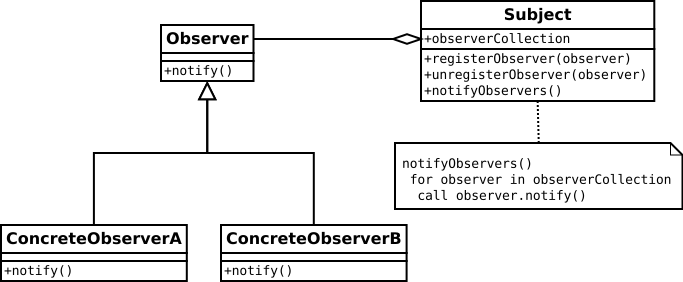
\includegraphics[width=0.8\linewidth]{images/Observer.pdf}
		\caption{UML Diagramm eines generischen Observer Patterns\cite{rmi-tutorial}}
		\label{broker}
	\end{center}
\end{figure}

\subsubsection{IDL}
Die Interface Definition Language ist eine deskriptive Sprache zur Definition von Sprachunabh\"angigien Interfaces.
Mittels eines IDL Compiles k\"onnen aus einer IDL Datei Stubs/Skeletons f\"ur die jeweilige Sprache generiert.
Im Falle des Chats sieht das IDL, welches eine ver\"anderte Version eines Tutorials von IBM ist, wie folgt aus:

\begin{lstlisting}[language={[CORBA]IDL}, caption=chat.idl]
#ifndef __CHAT_IDL__
#define __CHAT_IDL__
// this is a slightly adapted example of
// http://www.ibm.com/developerworks/webservices/library/co-corbajct3.html#h6
module chat {
    // Thrown by server when the client passes
    // an invalid connection id to the server
    exception InvalidConnectionIdException
    {
        long invalidId;
    };

    // This is the callback interface that
    // the client has to implement in order
    // to listen to a talker.
    interface Listener
    {
        // Called by the server to dispatch messages on the client
        void receive(in string message);
    };

    // interface on the server side
    interface Chatroom
    {
        // Called by the client to open a new connection
        // Returned long is the connection ID
        long register(in Listener client, in string listenerName);

        // Makes the server broadcast the message to all clients
        void send(in long connectionId, in string message) raises(InvalidConnectionIdException);

        // Called by the client to sever the communication
        void unregister(in long connectionId) raises (InvalidConnectionIdException);
    };
};
#endif // __CHAT_IDL__
\end{lstlisting}

Welches Interface, welcher Komponente des Observerpatterns entspricht ist relativ klar zu erkennen.
Ein \texttt{Chatroom} nimmt \texttt{Listener} Objekte entgegen und nimmt somit die Funktion des Subjects ein.
Au\ss erdem enth\"alt er die \texttt{send(...)} Methode zur Ver\"offentlichung von Nachrichten.

Ein \texttt{Listener} wird bei ankommenden Nachrichten vom \texttt{Chatroom} durch den Aufruf der \texttt{receive(...)} Methode benachrichtigt und nimmt somit die Funktion des Observers ein.

\subsubsection{Server}
Die Implementierung der Server erfolgt in Java.
Im ersten Schritt werden daf\"ur die Interface Definitionen mithife eines Ant-Tasks generiert:

\begin{lstlisting}[language=XML, caption=Ant Task f\"ur die Generierung der IDL Interfaces]
<property name="src.dir" value="src" />
<property name="build.dir" value="build" />
<property name="classes.dir" value="${build.dir}/classes" />
<property name="doc.dir" value="doc" />
<property name="idl.dir" value="../idl" />
<property name="gen.dir" value="${build.dir}/generated" />
<property name="resources.dir" value="resources" />
<property name="jacorb.dir" value="/home/markus/opt/jacorb" />

<!-- Setzen des Classpaths von JacORB -->
<path id="jacorb.classpath">

	<!-- Setzen des Pfades zu, und inkludieren der Libaries -->
	<fileset dir="${jacorb.dir}/lib">
		<include name="*.jar" />
	</fileset>
</path>

<!-- Setzen des Classpaths des Projekts (classes Ordner in build) -->
<path id="project.classpath">
	<pathelement location="${classes.dir}" />
</path>

<!-- Definieren eines in einer bestimmten Klasse vorhandenen Tasks -->
<target name="idl.taskdef">
	<taskdef name="jacidl" classname="org.jacorb.idl.JacIDL"
		classpathref="jacorb.classpath" />
</target>

<!-- Generieren des aus dem idl File resultierenden Quellcodes  -->
<target name="idl" depends="idl.taskdef">
	<mkdir dir="${idl.dir}" />
	<jacidl srcdir="${idl.dir}" destdir="${gen.dir}" includes="*.idl"
		helpercompat="jacorb" includepath="${jacorb.dir}/idl/omg" />
</target>
\end{lstlisting}

In dem Ant-Script wird durch den entsprechenden Aufruf des JacORB IDL Compilers die Stubs und Skeletons des Interfaces generiert.

Danach muss am Server Chatroom implementiert werden, dies erfolgt durch Vererben der Klasse \texttt{ChatroomPOA}.
In dem Code finden sich keine speziellen, Corba spezifischen Elemente, es handelt es sich um eine simple Methoden, welche keine besondere Aufmerksamkert bef\"urfen.

Interessanter ist jedoch die tats\"achliche Implementierung des Server und die Anbindung an Corba:
\begin{lstlisting}[language=Java, caption=Server Main Methode]
public static void main(String[] args)  {
    try {
        // Initialize the ORB
        ORB orb = ORB.init(args, null);
        System.out.println("Initialized ORB");

        //Instantiate Servant and create reference
        POA rootPOA = POAHelper.narrow(orb.resolve_initial_references("RootPOA"));
        ChatroomImpl chImpl = new ChatroomImpl();
        rootPOA.activate_object(chImpl);
        Chatroom chRef = ChatroomHelper.narrow(rootPOA.servant_to_reference(chImpl));

        //Bind reference with NameService
        NamingContext namingContext = NamingContextHelper.narrow(orb.resolve_initial_references("NameService"));
        System.out.println("Resolved NameService");
        NameComponent[] nc = { new NameComponent("Chatroom", "") };
        namingContext.rebind(nc, chRef);

        //Activate rootpoa
        rootPOA.the_POAManager().activate();

        //Start readthread and wait for incoming requests
        System.out.println("Server ready and running ....");

        orb.run();
    }	catch (Exception e)	{
        System.err.println("Es ist ein Fehler aufgetreten: " + e.getMessage());
        e.printStackTrace();
    }
}
\end{lstlisting}

In dem oberen Listing wird zun\"achst der ORB initalisiert und eine Referenz auf den Portable Object Adapter (POA) erzeugt, mithilfe dessen anschlie\ss end eine Instance von \texttt{Chatroom} als Objektreferenz an den Namensdient gebunden werden kann.
Dies geschieht in den Zeilen 7 bis 20.
Danach wird der ORB mit \texttt{orb.run()} gestartet.

Auch f\"ur die Ausf\"uhrung des Servers gibt es einen Ant-Task, welcher mit \texttt{ant run-server} gestartet.

\subsubsection{Client}
